\PassOptionsToPackage{svgnames}{xcolor}
\documentclass[10pt,letterpaper]{article}
\usepackage[top=.25in, bottom=.5in, left=.5in, right=.5in]{geometry}
\usepackage{tcolorbox}
\usepackage{lipsum}
\tcbuselibrary{skins,breakable}
\usetikzlibrary{shadings,shadows}

\usepackage{graphicx} % Allows to include images
\usepackage{booktabs} % Allows the use of \toprule, \midrule and \bottomrule in tables

\usepackage{multicol}
\usepackage{float}

\usepackage[T1]{fontenc}
\usepackage[utf8]{inputenc}

\title{Practice 1: The Introduction}
\author{}
\date{}

\newenvironment{agendablock}[1]{%
    \tcolorbox[beamer,%
    noparskip,breakable,
    colback=LightGray,colframe=DarkGray,%
    colbacklower=Gray!75!LightGray,%
    title=#1]}%
    {\endtcolorbox}

\newenvironment{evenBlock}[1]{%
    \tcolorbox[beamer,%
    noparskip,breakable,
    colback=LightGreen,colframe=DarkGreen,%
    colbacklower=LimeGreen!75!LightGreen,%
    title=#1]}%
    {\endtcolorbox}

\newenvironment{oddBlock}[1]{%
    \tcolorbox[beamer,%
    noparskip,breakable,
    colback=LightBlue,colframe=DarkBlue,%
    colbacklower=DarkBlue!75!LightBlue,%
    title=#1]}%
    {\endtcolorbox}

\newenvironment{myexampleblock}[1]{%
    \tcolorbox[beamer,%
    noparskip,breakable,
    colback=LightGreen,colframe=DarkGreen,%
    colbacklower=LimeGreen!75!LightGreen,%
    title=#1]}%
    {\endtcolorbox}

\newenvironment{myalertblock}[1]{%
    \tcolorbox[beamer,%
    noparskip,breakable,
    colback=LightCoral,colframe=DarkRed,%
    colbacklower=Tomato!75!LightCoral,%
    title=#1]}%
    {\endtcolorbox}

\newenvironment{myblock}[1]{%
    \tcolorbox[beamer,%
    noparskip,breakable,
    colback=LightBlue,colframe=DarkBlue,%
    colbacklower=DarkBlue!75!LightBlue,%
    title=#1]}%
    {\endtcolorbox}

\usepackage{lmodern}

\begin{document}
\fontfamily{lmss}\selectfont
\maketitle

\begin{agendablock}{Practice Activities}
    \begin{enumerate}
        \item Warm ups [ 10 min ]
        \item Coerver Touches, Sprinting with Ball (introduction) [ 20 min ]
        \item Query about desired positions [ 2 min ]
        \item Discuss new rules for U11 [ 3 min ]
        \item Roll Play Game Situations/Positioning (intro) [ 20 min ]
        \item Small Sided Game (position evaluation) [ 15 min ]
        \item Sprints [ 5 min ] 
    \end{enumerate}

\end{agendablock}

\section{Warm Up}

\begin{myalertblock}{Warm Ups (10 min) }
    \begin{enumerate}
        \item Jog to the 18 yard line and back twice with your ball (inside cut first time, outside cut the second),
        \item Side-Step to 18 yd line and back twice,
        \item Butt Kickers to the 18 yd line and back twice,
        \item Jog Backwards to the 18 yd line and back twice.
    \end{enumerate}
\end{myalertblock}

\begin{evenBlock}{Coerver Touches - Intro (20 min) }
    \begin{enumerate}
        \item Toe-Touches (20 count alternating feet): focus on speed, on your toes at all times.
        \item Pull back and Push: Pull the ball back with sole and push it forward with your laces. ( 10 count each foot).
        \item Side to Side or Pendulums: move ball from right foot to left foot with inside of the feet. ( 20 count )
        \item Triangle: ball starts in front of right foot, pull back and right pushes ball to the left.  Left foot pushes ball in front of the right foot, then repeat. (10 count)  Then switch feet for another 10 count (ball starts in front of left foot).
        \item Pullback-Behind: ball starts in front of right foot, pull back past the planted left foot.  Right then pushes the ball to the left behind the plant foot.  Player turns his body 90 degrees, takes one step to the ball then using his left foot pulls back the ball behind the planted foot and then pushes the ball behind the right foot.  Player turns 90 degree to the right, takes one step forward and repeats this sequence for 10 counts.
    \end{enumerate}
\end{evenBlock}

\begin{oddBlock}{Expectations}
    \begin{itemize}
        \item - Honesty \& Integrity:  Be honest and follow through on what you say you are going to do or promise.  If you do, nobody will question you and nobody will fault you when outcomes do not turn out as you expected because they will know you did everything you tried to do.
        \item Sportsmanship:  Discuss that this is team sport, there is no individual failure, we win and lose as a team.  Support each other, help each other and the other team to their feet.  If they are offer a quick check, then walk away and take a knee, clap and applaud them when they get up.
        \item Positive Attitudes: Do not spread negativity - it impacts everyone.  You don't need to be happy, but do not bring complaint or give up, stay positive and strive to learn from both good and bad outcomes.
        \item Work Hard: come ready to give it 100\% all the time.  We all have bad days, but you will grow more by giving it your all on a bad day than on a good day.
        \item Listen and Respect: everyone needs to be listening when a coach, the manager or a referee is talking to the team and give your respect to coaches, the team manager, the referee and the fans.  Bad language or attitudes will not be tolerated.
        \item If you care not to abide by these rules, we will practice for the track team - in other words you will be running a lot.
    \end{itemize}
\end{oddBlock}

\begin{evenBlock}{U11 Rules (5 min)}
    \begin{itemize}
        \item Larger field.
        \item Goal Keeper punts are now allowed.
        \item No retreat to half field.
        \item Offsides (explain this for the new boys).
        \item Throw-ins.
        \item 9 players not 7.  Introduce the 1-4-3-1  and 1-3-2-3 formations.
    \end{itemize}
\end{evenBlock}

\begin{oddBlock}{Basic Tactics}
    \begin{itemize}
        \item Movement without the Ball:
        \begin{itemize}
            \item Be in an open, reachable space.
            \item Play your role and position.  You may find saying your position over and over in your head makes you more aware of where you need to be.
            \item Be aware of your surroundings. Look around you constantly and mentally noting where open space is and what you could do next.
            \item Insure the player with the ball as at least 2 passing options.
            \item Communicate with your team if you see something out of place.  Look out for each other - we are a team.
        \end{itemize}
        \item When Ball is on our half:
        \begin{itemize}
            \item Push the play or take the play to the outside (to the sidelines).
            \item Never cross the ball in front of our goal.  Keepers - this includes you.  Move to the side you want to distribute before you distribute the ball.
            \item If a player is wide open in the center arc you can pass it there, however if the side line as an equally open player the side line is option 1.
        \end{itemize}
        \item Pass the ball forward.
        \item Passing the Ball Backward is frowned upon for a few reasons:
        \begin{itemize}
            \item A pass backward needs to be perfect - perfect location and pace.
            \item A bad backward pass gives the other team a greater advantage than loss of a possession due to a bad forward pass.
            \item A backward pass forces our team to switch directions (back petal) while the other team is able to continue to advance on the ball without losing pace.
        \end{itemize}
        \item Use the sideline to our advantage. Passing the ball down field to a player in the correct position will result in then handling inbounds or possibly the other team kicking it out - result we get a throw in that much closer to their goal, we maintain the advantage.
        \item Pass away from the previous pressure.
    \end{itemize}
\end{oddBlock}

\begin{evenBlock}{Funnel Positioning}
    Layout a few cones to demonstrate the physical location of the funnel on the field and walk through the positional plays, when the ball starts at our our keeper for a second time, but this time have the boys make decisions.
\end{evenBlock}

\section{Role Playing game Situations}

\begin{oddBlock}{Keeper Distribution}
    \begin{itemize}
        \item Distribute to one of the Outside Defensive Backs,
        \item Outside Midfielder Should be on sideline, body in an open stance, ready for the pass from the D-Back.
        \item The Midfielder then should then drive the ball down to the end line or look for a cross to the center forward or center midfielder.
        \item If midfielder makes the run to the end line the striker and opposite side midfielder need to make runs to position themselves for a potential cross. 
        \item If mid-fielder is able to penetrate deep, he should either cross the ball or pass the ball back to the advancing outside D-back now playing a mid-fielder position.
        \item  A cross should result in a shot attempt.  If the cross is blocked its likely to cross the end line resulting in a corner kick.
        \item The less preferred option is a pass backward to the supporting outside D-back.  The D-Back should play the ball quickly to the far sideline mid-fielder or outside D-back or center mid-fielder (who should them play it to the side line or drive it that direction).
    \end{itemize}
\end{oddBlock}

\begin{evenBlock}{Defensive Positioning}
    On the Other Teams Half:
    \begin{itemize}
        \item Push them to the center of the field.
        \item Forwards and Outside Mid-Fielders need to be aggressive.  Attack the ball.
        \item Defensive backs and center mid-fielder be more conservative, shuddle backward and attack the ball when the Offensive player is off balance or making a move.
    \end{itemize}
    If ball crosses into our half:
    \begin{itemize}
        \item Force them to the outside.
        \item Play more conservatively until you have support, then be aggressive.
        \item Remember the funnel - position yourself correctly.
        \item Center D-backs are the last line of defense.  If they are in play, forwards and mid fielders need to be racing in to support the defense.
    \end{itemize}
\end{evenBlock}

\begin{oddBlock}{Try It}
    Let the boys run the plays without defenders from both sides.
\end{oddBlock}

\section{Game}

\begin{evenBlock}{Small Sided Game (15 min)}
    Play a small sided game.  Keepers may be optional. Move the boys around and evaluate each one for good role fits.
\end{evenBlock}

\section{Close}
\begin{oddBlock}{Sprints}
    Agility runs to cone 5 yards away, stop and step circling cone then explode to next cone, circling it then explode sprinting to half field, jog back to end line and repeat 3 times.
\end{oddBlock}
%\begin{oddBlock}{Role Playing game Situations}
%
%\begin{minipage}[t]{\linewidth}
%    \centering
%    
%    \begin{minipage}{.3\linewidth} % Left column and width
%        %\begin{figure}
%            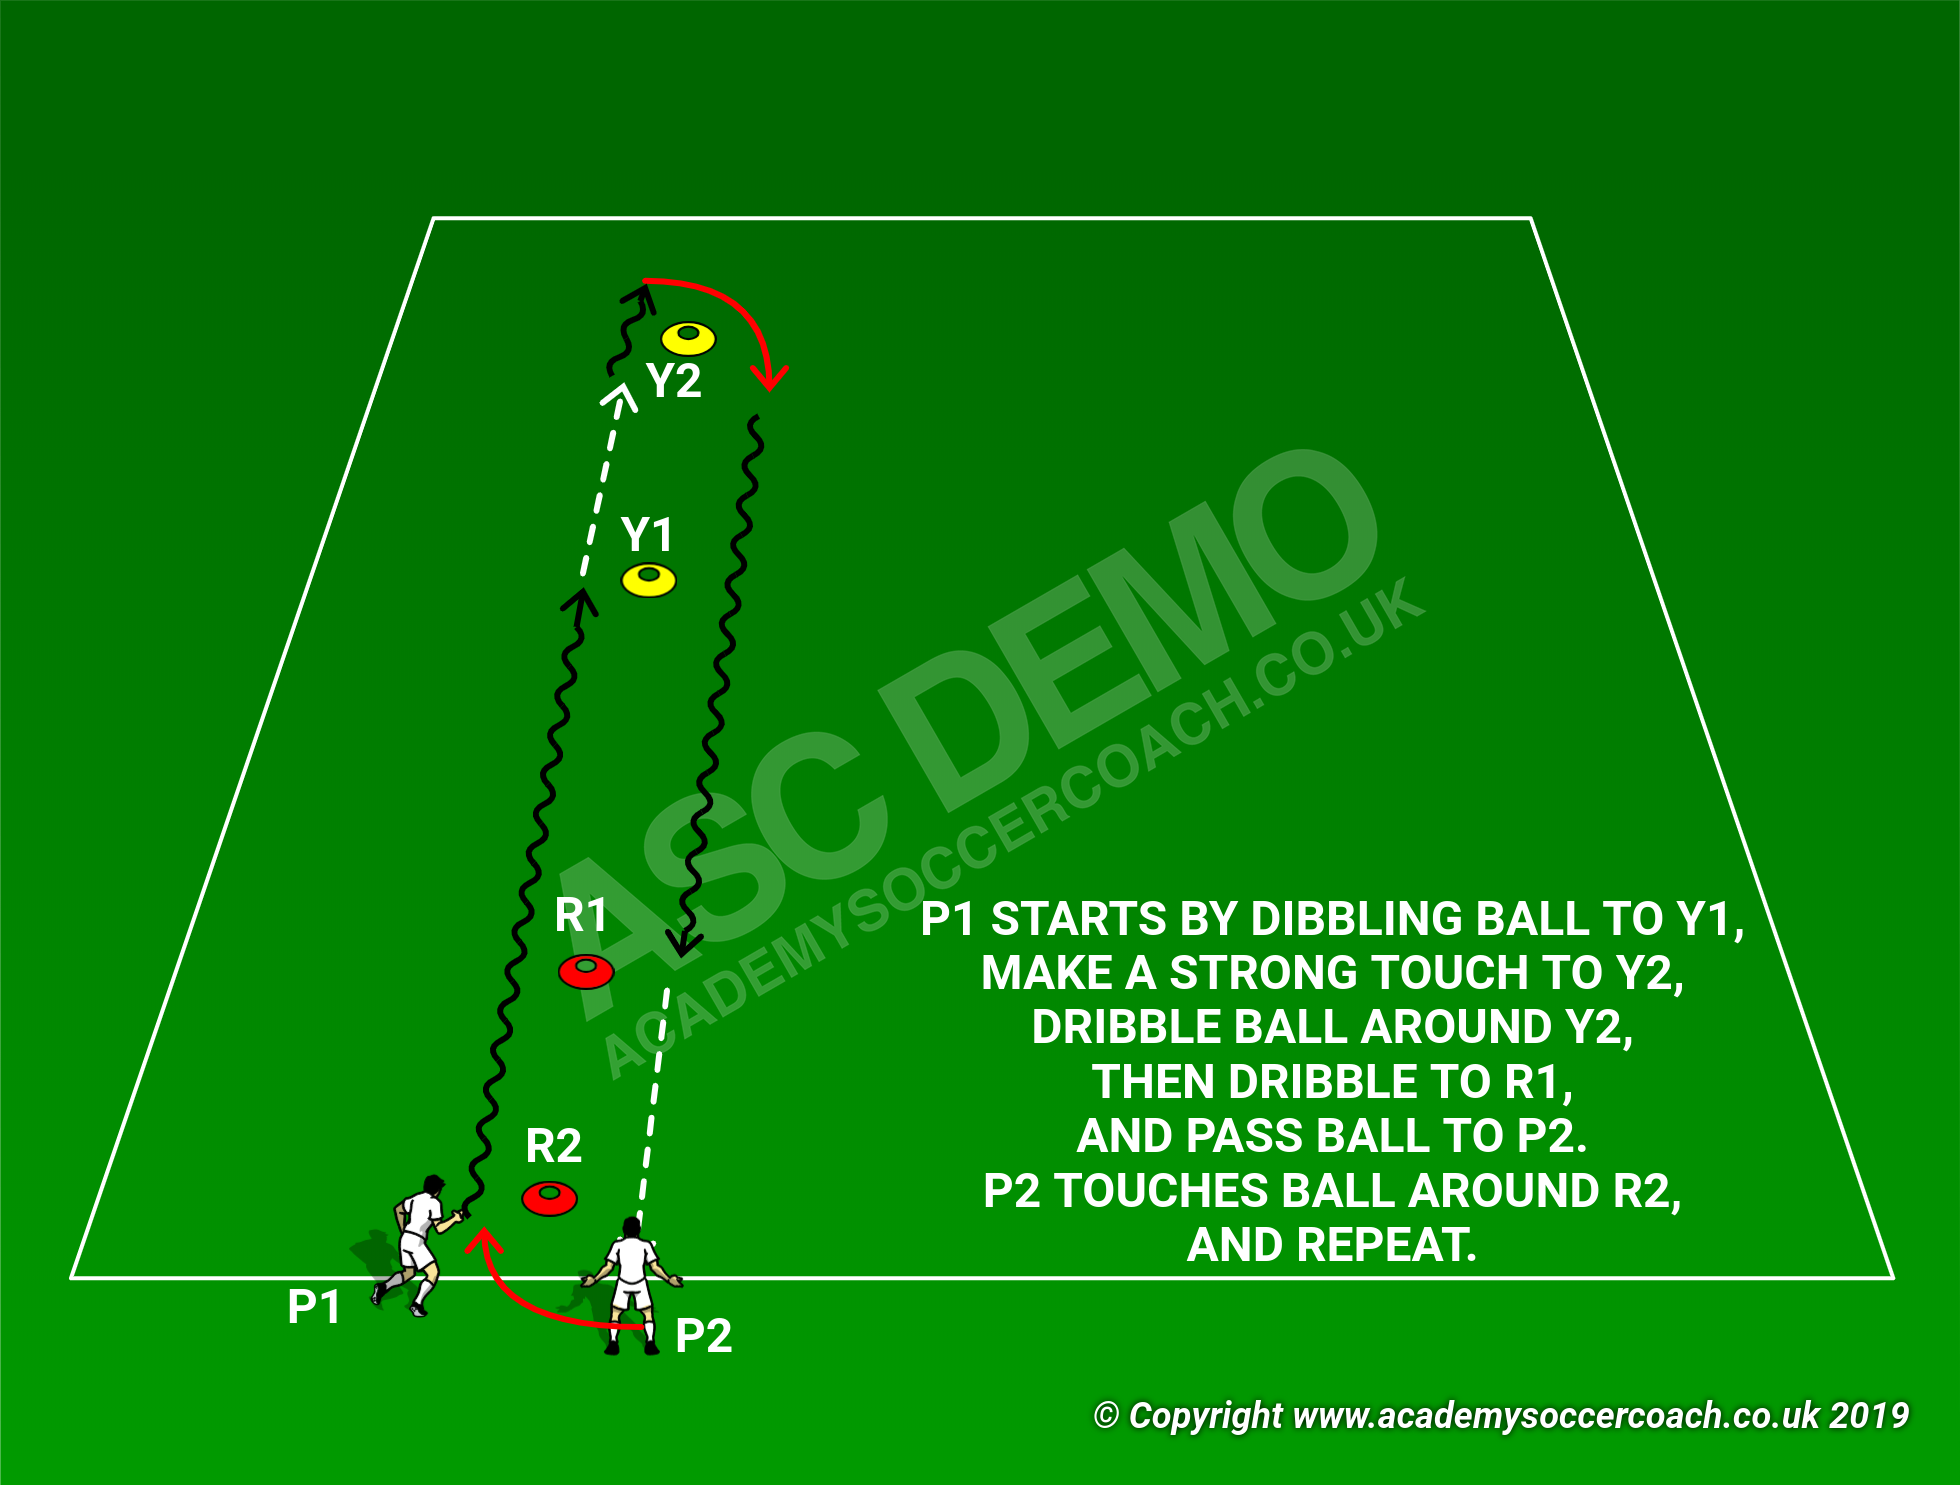
\includegraphics[width=\textwidth]{../img/Play1.png}
%        %    \caption{Drill: 4 Person Passing}
%        %\end{figure}
%    \end{minipage}
%    \hspace{0.05\linewidth}
%    \begin{minipage}{.6\linewidth} % Left column and width
%        \textbf{Drill Description:}
%        \begin{enumerate}
%        \setlength{\itemsep}{0pt}
%        \setlength{\parskip}{0pt}
%        \setlength{\parsep}{0pt}
%        \item First player passes using his right foot to the player on his left.
%        \item That player traps the ball with his left foot and passes with his right.
%        \item Play continues for half the time, before switching directions and feet.
%        \end{enumerate}
%
%        \textbf{Coaching Points:}
%        \begin{itemize}
%        \setlength{\itemsep}{0pt}
%        \setlength{\parskip}{0pt}
%        \setlength{\parsep}{0pt}
%        \item Receive the ball on the correct foot!
%        \item Be on your toes and move to make the first touch on the correct foot!
%        \item Body position needs to be open - allowing you to see the other three players at ALL times.
%        \item Make a strong accurate pass.
%        \end{itemize}
%
%    \end{minipage}
%\end{minipage}
%
%\end{oddBlock}
%
%\begin{myexampleblock}{Example of \texttt{myexampleblock}}
%\lipsum[2]
%\end{myexampleblock}
%
%\begin{myalertblock}{Example of \texttt{myalertblock}}
%\lipsum[1]
%\end{myalertblock}

\end{document}